% SOURCE_AUTHORITY: sga5_fr_workpass.tex, lines 7941--8004 (LF-normalized unit).
% SOURCE_SHA256: 791F4EFFC5E02832D5D77ED03518C8156D6F07E4C8238B03545DB93D883FBB28
\subsubsection*{A.2. Caso dos sistemas projetivos}
Seja agora \(X=(X_n)_{n\in\mathbb Z}\) um sistema projetivo de objetos de uma categoria abeliana \(\mathcal C\), tal que
\[
X_i=0\qquad(i<0).
\]
Se \(T\) denota um \(\delta\)-funtor exato de \(\mathcal C\) em uma categoria abeliana \(\mathcal D\), \(T\) se prolonga naturalmente a um \(\delta\)-funtor exato, ainda denotado por \(T\):
\[
\Hom(\mathbb Z^\circ,\mathcal C)\longrightarrow \Hom(\mathbb Z^\circ,\mathcal D).
\]
Assim, dotando \(X\) de sua filtração natural de sistema projetivo (EGA \(0_{\mathrm{III}}\) 13.4.1), obtém-se uma sucessão espectral:
\[
\mathbb E(X)=\mathbb E(X_n)_{n\in\mathbb Z},
\]
onde os \(\mathbb E(X_n)\) denotam as sucessões espectrais associadas a \(T\) e a \(X_n\) com filtração induzida.

\paragraph{Propriedades de \(\mathbb E(X)\).}
a) Para todo inteiro \(n\), a filtração do termo limite \(E^n(X)\) na sucessão espectral \(E(X)\) coincide com sua filtração natural de sistema projetivo quando \(X\) é estrito.

Com efeito, denotando pela letra \(F\) (como em A.1) a primeira filtração e pela letra \(\Phi\) a segunda, tem-se, para todo inteiro \(\alpha\):
\[
F^pE^n(X)_\alpha
=\Ker\bigl(T^n(X_\alpha)\longrightarrow T^n(X_\alpha/F^pX_\alpha)\bigr)
\]
\[
=
\begin{cases}
0,& \alpha\le p-1,\\
\Ker\bigl(T^n(X_\alpha)\longrightarrow T^n(X_{p-1})\bigr),& \alpha\ge p-1.
\end{cases}
\]
Em ambos os casos, é reconhecida a expressão \(\Phi^pE^n(X)\).

Isto mostra, em particular, que, para \(\beta\ge\alpha\ge p\), o morfismo de transição
\[
E_\infty^{pq}(X_\beta)\longrightarrow E_\infty^{pq}(X_\alpha)
\]
que se identifica com
\[
\gr_T^pT^{p+q}(X_\beta)\longrightarrow
\gr_T^pT^{p+q}(X_\alpha),
\]
é um monomorfismo, por EGA \(0_{\mathrm{III}}\) 13.4.1.3.

b) Fixado \(\alpha\in\mathbb Z\), é claro (cf. a figura anexa) que, uma vez que \(F^i(X_\alpha)=0\) para \(i\ge\alpha+1\), tem-se:
\[
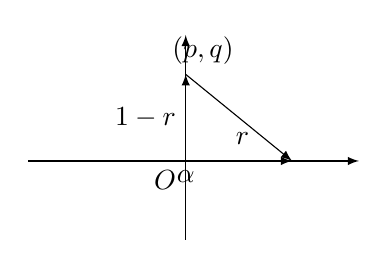
\begin{tikzpicture}[baseline=(current bounding box.center),x=1.0cm,y=1.0cm,>=latex]
\draw[->] (-2.0,0) -- (2.2,0);
\draw[->] (0,-1.0) -- (0,1.6);
\node[below left] at (0,0) {$O$};
\node[below] at (0,0) {$\alpha$};
\draw[->] (0,0) -- (0,1.1);
\draw[->] (0,1.1) -- (1.35,0);
\draw[->] (0,0) -- (1.35,0);
\node[above] at (.22,1.1) {$(p,q)$};
\node[left] at (0,0.55) {$1-r$};
\node[above] at (.72,0.08) {$r$};
\end{tikzpicture}
\]
\[
B_r^{pq}(X_\alpha)=B_{r+1}^{pq}(X_\alpha)\quad\text{para }r>p,
\]
\[
Z_r^{pq}(X_\alpha)=Z_{r+1}^{pq}(X_\alpha)\quad\text{para }r>\alpha-p.
\]
